\documentclass[11pt]{article}
\usepackage{geometry}
\usepackage{amsmath}
\usepackage{amssymb} 
\usepackage{color}
\usepackage{datetime}
\usepackage{everypage}
\usepackage{lastpage}
\usepackage{multirow}
\usepackage{textpos}
\usepackage{nicefrac}
\usepackage{setspace}
\usepackage{tikz}
\usepackage{lineno}
\usepackage{pifont}
\newcommand{\dblbkt}[1]{}
\usetikzlibrary{calc,arrows,automata,shapes.misc,shapes.arrows,chains,matrix,positioning,scopes,decorations.pathmorphing,shadows}
%can always use
\topmargin 0in 
\headheight 0in 
\headsep 0in 
\textheight 9in 
\textwidth 6.5in 
\oddsidemargin 0in 
\evensidemargin 0in 

\setlength\TPHorizModule{1in}
\setlength\TPVertModule{1in}

\pagestyle{empty}
\settimeformat{ampmtime}
\begin{document}

\makeatletter
\def\makeLineNumberLeft{%
  \linenumberfont\llap{\hb@xt@\linenumberwidth{\LineNumber\hss}\hskip\linenumbersep}% left line number
  \hskip\columnwidth% skip over column of text
  \rlap{\hskip\linenumbersep\hb@xt@\linenumberwidth{\hss\LineNumber}}\hss}% right line number
\leftlinenumbers% Re-issue [left] option
\makeatother


\linenumbers


\AddEverypageHook{
  \begin{textblock}{8.5}(-1,-1) 
    \textblockcolour{}
    \begin{tikzpicture}[transform shape,>=stealth] 
      \hspace{-.05in}
      \node at (0in,0in){};
      \node at (8.5in,-11in){};
      \def\topbar{-.5in}
      \def\bottombar{-10.25in}
      \draw (.5in,\bottombar) -- (8in,\bottombar);
      \node [anchor=north] at (4.25in,\bottombar) {};
      \node [anchor=north west] at (.5in,\bottombar) {};
      \node [anchor=south] at (4.25in,\topbar) {Vernon Smith Experimental Economics Laboratory $ \bullet $ Purdue University };
      \draw (.5in,\topbar) -- (8in,\topbar);
      \node [anchor=north] at (4.25in,\bottombar-.1in) {Page \thepage\ };%of \pageref{LastPage}};
      \node [anchor=south east] at (8in,\topbar) {};
      \node [anchor=south west] at (.5in,\topbar) {};
    \end{tikzpicture}
  \end{textblock}
}

%STARTTEXT


\def\firstChoice{W}
\def\secondChoice{Y}
\def\numberOfMatches{ten}
\def\exchangeRate{1250}
\def\costAmount{0}
\def\quizFirstAttempt{0.75}
\def\quizSecondAttempt{0.25}
\def\quizBonusAll{2.50}
\def\quizMaxTotal{10.00}

\vspace{-.5in} 



\section*{\dblbkt{3} Experiment Overview \dblbkt{slnc 500}} 

You are about to participate in an \dblbkt{1} experiment in the economics of decision-making. If you listen carefully, \dblbkt{1} you could earn a large amount of money, that will be paid to you in cash, in private, at the end of the experiment. 
\\ 
\\ 
It is important \dblbkt{1} that you remain silent and do not look at other people's work.  If you have any questions, or need any assistance of any kind, \dblbkt{1} please raise your hand and an experimenter will help you out. \dblbkt{3} During the experiment, \dblbkt{1} {\bf do not talk, laugh or exclaim out loud} and be sure to \dblbkt{1} keep your {\bf eyes on your screen only}.  In addition, \dblbkt{1} please {\bf turn off your cell phones, etc.} and put them away during the experiment.  Anybody that violates these rules will be asked to leave and will {\bf not} be paid. \dblbkt{1} We expect, and appreciate your cooperation. 

\subsection*{\dblbkt{3} Agenda}
\begin{enumerate} 
\dblbkt{1} \item We will first go over the instructions.
\dblbkt{1} \item Then we will have a practice match to learn the interface. 
\dblbkt{1} \item Next, there will be a quiz with 10 questions to make sure everyone understands the instructions. \dblbkt{slnc 1000}
\begin{itemize}
\dblbkt{1} \item All 10 questions will refer to these instructions so you should follow them carefully.
\dblbkt{1} \item If you answer {\bf all questions correctly you will earn \$\quizMaxTotal}. \dblbkt{slnc 1000}  
\dblbkt{1} \item If you answer {\bf at least one question incorrectly you will earn \$0}, at which point you will not need to answer any more questions. \dblbkt{slnc 1000}
\dblbkt{1} \item You will have 10 minutes to answer the 10 questions.
\end{itemize} 
\dblbkt{1} \item After the quiz, you will have 10 minutes to prepare for the experiment. \dblbkt{3} In the experiment you will be working with a fictitious currency called Francs. You will be paid in US Dollars at the end of the experiment. \dblbkt{1}  {\bf The exchange rate today is: \underline{\exchangeRate} Francs = \underline{1.00} USD.} \dblbkt{slnc 4000}
\end{enumerate} 


\section*{\dblbkt{3} Experiment Details} 
\begin{itemize} 
\item \dblbkt{1} This experiment consists of {\bf \numberOfMatches}  matches. 
\item \dblbkt{1} Prior to start of the experiment, all participants may be split into two groups. The groups will stay fixed and you will know the number of participants in your group throughout the experiment.
\item \dblbkt{1} At the beginning of each match, you will be paired {\bf randomly} with one other participant from your group.  You will remain {\bf matched with this same participant until the  end of the match}, but then will be paired with another randomly selected participant from your group in the following match.
\item Each match will have the same structure, \dblbkt{1} but may contain different numbers of periods. 
\item \dblbkt{1} You will remain {\bf anonymous throughout the experiment}.  You will not know the identity of the participant that you are paired with, and they will not know your identity. \dblbkt{1} The choices made by you, and the participant you are paired with, have no effect on the payoffs of participants in other pairs, and vice versa. Therefore, {\bf your payoff in a given match is based solely on the choices made by you and the participant that you are paired with}.
\item \dblbkt{5} Next, Let's Look at the experimental Interface \dblbkt{slnc 2000}
\end{itemize}


\section*{Specific Instructions for Each Period} 


\begin{itemize} 
\item Your payoff in each period will depend on your choice and the choice of the participant that you are paired with. 
\item You will choose one of two options, either $\firstChoice$ or $\secondChoice$.
\item You will be able to see the payoffs for each combination of choices for you and the participant that you are paired with. 
\item These payoffs will remain the same throughout the entire experiment (all matches).
\item \dblbkt{2} The payoffs will be displayed in a table like this:


\begin{center} 
	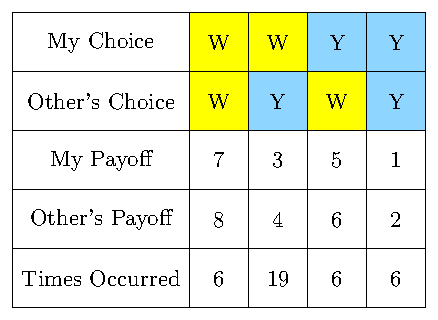
\includegraphics[width=3in]{pictures/gameTable_Reverse.pdf} 
\end{center} 

In this example above, the rows are the following:
\begin{itemize} 
\item \dblbkt{1} Row \#1 - Your choice (either $\firstChoice$ or $\secondChoice$ in this example)
\item \dblbkt{1} Row \#2 - Other's choice (either $\firstChoice$ or $\secondChoice$ in this example).
\item \dblbkt{1} Row \#3 - Your payoff.
\item \dblbkt{1} Row \#4 - Other's payoff.
\item \dblbkt{1} Row \#5 - Total number of times that that combination has been played {\bf this match}.
\end{itemize} 

{\bf Examples:}
\item In the table above, \dblbkt{1} if you choose $\firstChoice$ and \dblbkt{1} the participant that you are paired with chooses $\secondChoice$, then \dblbkt{1} you receive a payoff of 3, and \dblbkt{1} the participant that you are paired with receives a payoff of 4.  \dblbkt{1} This combination has occurred 19 times so far this match. 
\item \dblbkt{1} If you choose $\firstChoice$ and \dblbkt{1} the participant that you are paired with chooses $\firstChoice$, then \dblbkt{1} you receive a payoff of 7, and \dblbkt{1} the participant that you are paired with receives a payoff of 8.  \dblbkt{1} This combination has occurred 6 times so far this match.
\item \dblbkt{1} If you choose $\secondChoice$ and \dblbkt{1} the participant you are paired with chooses $\secondChoice$, then \dblbkt{1} you receive a payoff of 1, and \dblbkt{1} the participant that you are paired with receives a payoff of 2.
 \dblbkt{1} This combination has occurred 6 times so far this match.
\end{itemize}

\subsection*{\dblbkt{3} History}

\begin{itemize} 
\item As the match progresses, you will see the {\bf history} of play across the top of the screen, displayed like this: \dblbkt{2}

\hspace{-1in}
  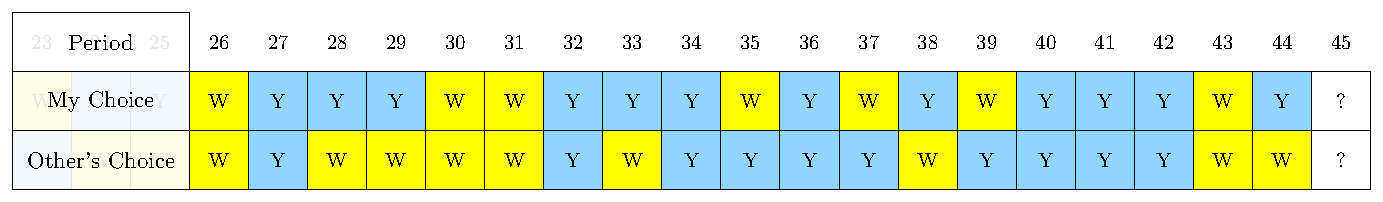
\includegraphics[width=7.5in]{pictures/history.pdf} 
\item This history displays \dblbkt{1} the period (labeled Period), \dblbkt{1} your choice in that period (labeled {\bf My Choice}), \dblbkt{1} the choice of the participant you are paired with in that period (labeled {\bf Other's Choice}), and \dblbkt{1} the payoff for that period (labeled My Payoff). 
\item For example, in the above history, \dblbkt{1} in period 39, \dblbkt{1} you played $\firstChoice$, \dblbkt{1} the participant you are paired with played $\secondChoice$, \dblbkt{1} and you received a payoff of 3.
\end{itemize} 



\subsection*{\dblbkt{2} Rules}
\begin{itemize} 
\item Rather than directly making choices of $\firstChoice$ or $\secondChoice$, you will develop a set of rules which will automatically make choices for you. 
\item \dblbkt{3} The set of rules will appear in the middle of the screen. 
\item \dblbkt{3} You will be able to construct rules using the rule constructor at the bottom of the screen.
\item \dblbkt{3} A rule consists of two parts:
\begin{itemize} 
\item \dblbkt{1} {\bf Input Sequence} - A sequence of choices made by you and the participant you are paired with. 
\item \dblbkt{2} {\bf Output} - A choice to be made by you after the input sequence occurs. 
\end{itemize} 

\item \dblbkt{2} Some example rules are displayed below:
  
\begin{tabular}{ccc} 
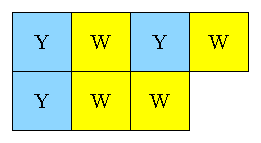
\includegraphics[height=1in]{pictures/rule1.pdf} & 
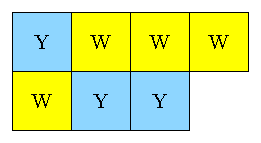
\includegraphics[height=1in]{pictures/rule7.pdf} & 
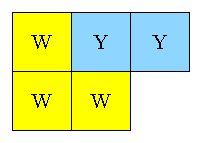
\includegraphics[height=1in]{pictures/rule4.pdf} \\ 
Rule \#2 & Rule \#3 & Rule \#4
\end{tabular} 

\item \dblbkt{1} For example, Rule \#2 has an input sequence of \dblbkt{1} ($\secondChoice$,$\secondChoice$), \dblbkt{1}($\firstChoice$,$\firstChoice$), \dblbkt{1}($\secondChoice$,$\firstChoice$) and an output of \dblbkt{1}$\firstChoice$.  This means that if you have played \dblbkt{1}$\secondChoice$, $\firstChoice$, and then $\secondChoice$ in the last three periods, and the participant that you are paired with has played \dblbkt{1}$\secondChoice$, $\firstChoice$, and then $\firstChoice$, this rule will lead you to play \dblbkt{1}$\firstChoice$ in the next period.


\item As play progresses you will develop a set of rules that will be used to make your choices. Play will proceed as follows:  
\begin{itemize}
\item Each period, \dblbkt{1}your set of rules will select the choice to be made next period. 
\item The \dblbkt{1} rule that will be used to make the choice will be highlighted.
\item The corresponding \dblbkt{1} sequence in the history will be highlighted.
\item A \dblbkt{1} preview of the choice to be made next period will be shown as a lightly colored cell on the history of play.
\item In order to move to the next period, {\bf you have to confirm the choice by clicking on the corresponding history cell.}  \dblbkt{1}Once you have confirmed your choice, the light color will turn to a regular color, and you may need to wait for the participant that you are paired with to make their choice. \dblbkt{slnc 5000}\dblbkt{1}
\end{itemize}


\item There are several ways that you can modify your rules during the experiment.  
\begin{enumerate} 
\item \dblbkt{1}First, you can use the rule constructor in the bottom center of the screen. \dblbkt{1}Press the plus button to add more columns, \dblbkt{1}or one of the minus buttons to subtract columns.  Click on the question marks to fill in the boxes.  When you click on a question mark, \dblbkt{1}either a $\firstChoice$ or a $\secondChoice$ will appear.  If you click on a $\firstChoice$, \dblbkt{1}it will switch to a $\secondChoice$, and if you click on a $\secondChoice$, \dblbkt{1}it will switch to a $\firstChoice$.  \dblbkt{1}Once you have completely filled in the rule (leaving no question marks), \dblbkt{1}the {\bf add rule} button will appear, \dblbkt{1}and the rule can be added to your set. 
\item Second, if you look at a rule in the set, \dblbkt{1}you will notice a green copy button, \dblbkt{1}and a red delete button.  If you \dblbkt{1}press the green {\bf copy button (\ding{112})}, it will copy the rule down to the constructor, \dblbkt{1}and you will be able to create a similar rule.\dblbkt{slnc 2000} If you \dblbkt{1}press the red {\bf delete button (\ding{56})}, it will delete the rule from the \dblbkt{1}set. \dblbkt{slnc 2000}
\item Since your rule set needs to make a single choice each period, it is not possible to have two rules with the same input sequence, but with different outputs.  \dblbkt{1}If you create a rule that has the same input sequence but a different output, you will get an error that \dblbkt{1}says {\bf ``Conflicting rule in set"}, and a \dblbkt{1}button that says {\bf ``Switch Rule"} will appear.  If you press this button, it will delete the \dblbkt{1}conflicting rule from the rule set, \dblbkt{1}and add the rule from the \dblbkt{1} constructor.  \dblbkt{slnc 2000}
\end{enumerate} 

\item The {\bf length of the rule} is measured by the length of the input sequence. 
\item So \dblbkt{1}rule \#2, and \dblbkt{1}rule \#3 have a length of 3, and \dblbkt{1}rule \#4 has a length of 2. 

\item A rule of length $n$ is said to {\bf fit the history} if the input sequence matches the last $n$ periods of the history. 
\item For example, since the last three periods of play in the above history \dblbkt{1}(periods 42-44) have been \dblbkt{1}$ \left( Y , Y \right)$, \dblbkt{1}$\left( W, W \right)$, and \dblbkt{1}$\left( Y , W \right) $, and that sequence is also the input for \dblbkt{1}rule \#2, \dblbkt{slnc 1000}then rule \#2 is said to fit the history.
Similarly, given the above history, we can see that \dblbkt{1}rule \#4 fits the history, \dblbkt{slnc 1000} but \dblbkt{1} rule \#3 does not fit the history.  

\item If more than one rule fits the history, then the {\bf rule with the longer length will determine the choice}.  
\item For example, given the above history since both \dblbkt{1}rule \#2, and \dblbkt{1}rule \#4 fit the history, \dblbkt{1}rule \#2 will be used to make your choice, since it is longer.  Therefore, given the history, and the rule set, your choice next period will \dblbkt{1}be $\firstChoice$, as prescribed by \dblbkt{1}rule \#2. \dblbkt{1} \dblbkt{slnc 2000}
\item If no rules fit the history, then your \dblbkt{1}{\bf Default Rule} will be selected.  The default rule will only be used when no rules fit the history. \dblbkt{1}To select your default rule select either \dblbkt{1}$\firstChoice$, or \dblbkt{1}$\secondChoice$, in the bottom left of your screen.

\item Additionally, you have to select the \dblbkt{1}{\bf First Period} rule. The first period rule will only be used in the first period of the match. To select your first period rule select either  \dblbkt{1}$\firstChoice$, or \dblbkt{1}$\secondChoice$, in the bottom left of your screen.  
\end{itemize} 

\subsection*{\dblbkt{1}Additional Examples}

 
 \hspace{-.5in}
  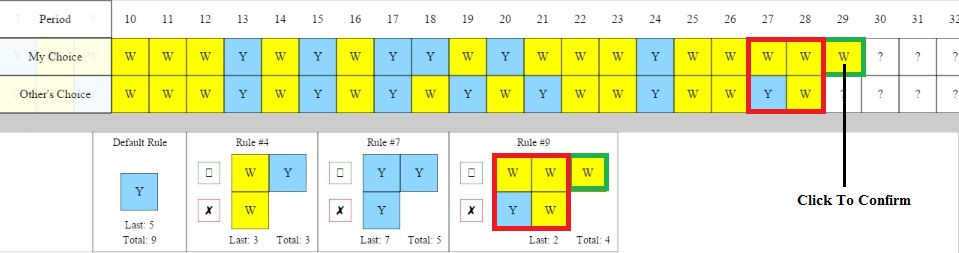
\includegraphics[width=7in]{pictures/q3sApr2016.jpg} 
\begin{itemize}
\item In the example above, \dblbkt{1}Rule \#4, and \dblbkt{1}Rule \#9, both {\bf fit} the history. However, rule \#9 will be selected because it is longer. Therefore, \dblbkt{1}$\firstChoice$ will be played in the next period, \dblbkt{1}as prescribed by rule \#9. 
\item For the example above, how can we change the rule set to ensure that $\secondChoice$ is played next period. There are several ways to make changes to the rule set in order for $\secondChoice$ to be played. First, you can {\bf delete (\ding{56})} \dblbkt{1}Rule \#9, which would cause \dblbkt{1}Rule \#4 to be the longest rule that fits the history, \dblbkt{1}and therefore would lead to $\secondChoice$ being played next period. \dblbkt{slnc 5000} \dblbkt{1}Second, you \dblbkt{1}can {\bf add a longer rule that fits the history} that has $\secondChoice$ as the output. Since you added a longer rule that fits the history, that rule will be used to make the choice, and will select $\secondChoice$ as the choice for next period.\dblbkt{slnc 5000} 
\end{itemize}


\subsubsection*{\dblbkt{4}Number of Periods Per Match} 

\begin{itemize} 
\item The number of periods in each match will be determined randomly using the following procedure.  
\begin{itemize} 
  \item At the end of each period, \dblbkt{1}a number will be chosen randomly from the set of numbers \dblbkt{1} $ \{1,2,3,\ldots,48,49,50\}$, where {\bf each number is equally likely}.  
  \item \dblbkt{1}If the number is 1, then the match will end.
  \item \dblbkt{1}If the number is not 1, then the match will continue.
  \item The number will always be placed back into the set after it is drawn.  
  \item Thus, in any period there is a 2\% CHANCE that the match will end, and a 98\% CHANCE that the match will have another period.
  \item Therefore, \dblbkt{1}the expected number of periods in each match will be 50.
  \item \dblbkt{2}This procedure has been performed on the computer before the experiment. Therefore, you will not see the number selected from $ \{1,2,3,\ldots,48,49,50\}$.
  \item To ensure that the length of the match is not dependent on your play, the number of periods for each match has be written on the board before the experiment, and will be uncovered at the end of the experiment.  
\end{itemize} 
\item \dblbkt{3}Your choices will be determined \dblbkt{1}automatically from your rule set. However, {\bf you will need to confirm the \dblbkt{1}choice within an allotted amount of time.} To confirm your choice, \dblbkt{1}click on your action for the next period within the history at the top of the screen. If you don't confirm the choice within the allotted amount of time, \dblbkt{1}then the choice will be confirmed automatically at the end of the allotted time. {\bf The experiment will not be able to proceed until everyone confirms their choices.}
\item \dblbkt{1}Everyone in your group will have the same amount of time allotted in each period. 
\end{itemize}

\subsubsection*{\dblbkt{3}Additional Information about Matches}
\begin{itemize} 
\item During matches 1-10 you will be able to construct the set of rules to make your choices.
\item \dblbkt{1}All of the rules in your set at the end of one match will remain in your set at the start of the next match.  
\item \dblbkt{1}Before the first match, \dblbkt{1}you will have 1 minute to look over the payoffs, \dblbkt{1}and an additional 10 minute to construct your rules.
\end{itemize} 


\subsubsection*{\dblbkt{5}Editing your set of rules}
\begin{itemize} 
\item In the experiment today you will need to {\bf pay a cost to edit rules during the match}.  
\item More specifically, 
\begin{itemize} 
\item {\bf Before each match starts,} you can make changes to your set of rules at no cost.
\item {\bf After each match starts,} if you want to make changes to your set of rules, \dblbkt{1}you must click the {\bf ``Unlock Rules"} button. The {\bf cost} for clicking the ``Unlock Rules" button is {\bf \costAmount\ Francs}.  The total cost incurred in all matches\dblbkt{1} will be displayed at the top of the screen in red. {\bf You will be able to edit your rules for the duration of one period.} Once you are done editing your rules you may click the {\bf ``Lock Rules"} \dblbkt{1}button.  
\item If you don't want to make changes to your set of rules, you may choose not to click the {\bf ``Unlock Rule"} button. Then you will not incur the cost of \costAmount\ Francs. 
\item In either case, {\bf you will need to confirm the choice made within the time limit set for each period.} 
\item If the time limit within a period is reached, your rules will become locked, your choice will be confirmed automatically, and you will proceed to the next period.
\end{itemize} 
% \item You can make changes to your rules before each match without incurring any costs. 
% \item If you want to make changes to your set of rules during the match you can click the {\bf``Edit Rules"} button. The {\bf cost} of editing your rules during the match is {\bf 25 points} for clicking the ``Edit Ruels" button plus {\bf 3 points per  second} that you are editing the rules. 
% \item Once you are done editing your rules you may click the {\bf ``Lock Rules"} button, after which point you will no longer incur any costs.
\end{itemize} 



\subsection*{\dblbkt{5}Starting Rules}
\begin{itemize} 
\item Prior to the start of the experiment {\bf you will have 10 minutes} to construct your starting set of rules.
\item During that time, you will be presented with a split-screen view of of the construction screen. In this view, you will have an opportunity to test what your rule set will select as an output for a variety of {\bf hypothetical histories}.
\item The split-screen will consist of two sides.  \dblbkt{1}The right side is the {\bf Starting Rules} side.  Rules added to this side will be added to your rule set at the start of the first match.   \dblbkt{1}The left side is the {\bf Hypothetical Rules} side.  Rules added to this side can be used to test to see what choices different combinations of rules will lead to.
\item  You will be able to move rules from the Hypothetical Rules side to the Starting Rules side \dblbkt{1}by clicking the blue {\bf move (\ding{222})} button. To delete rules from either side, \dblbkt{1}you need to click the {\bf delete (\ding{56})} button.
\item You will be able to see what choice \dblbkt{1}your hypothetical, and \dblbkt{1}your starting rule sets select as a choice for next period, for each of the {\bf hypothetical histories that you construct}.  
\item Notice that you will be able to construct, and store, {\bf multiple histories} \dblbkt{1}at the same time.  You can view one of the other hypothetical histories by clicking the \dblbkt{1}{\bf History \#} button at the top of the Hypothetical Rules side. You can add a new hypothetical history by clicking the \dblbkt{1}{\bf New} button at the top of the Hypothetical Rules side.  
\item  To construct  a hypothetical history you will need to click on the \dblbkt{1}question marks in that history.  You don't need to fill out the entire history to see what choice your rule set will make.  Therefore, it is useful to start filling out the new histories from the most recent periods on the right side. 

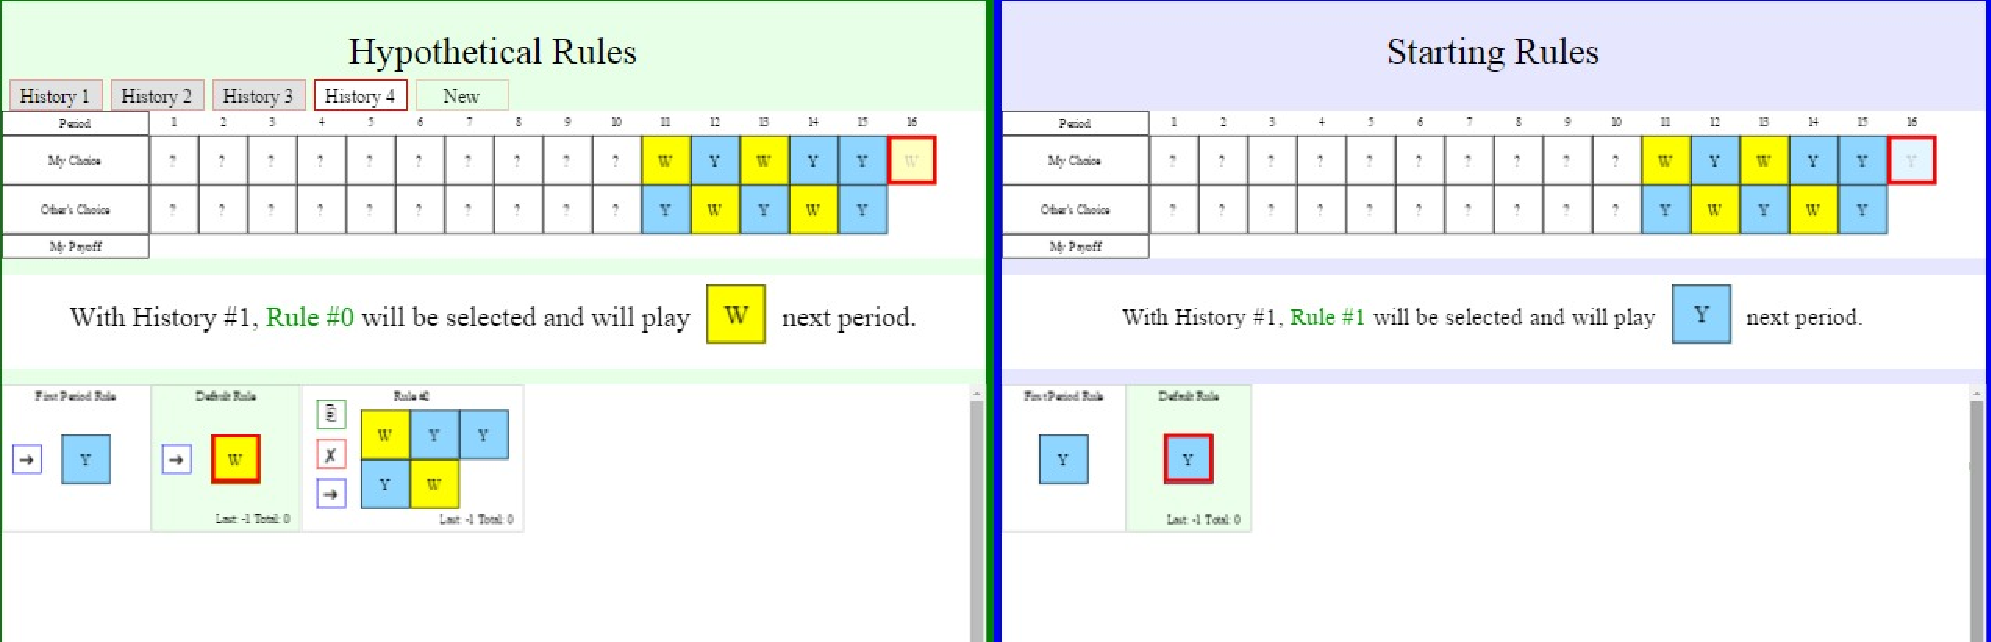
\includegraphics[width=6in]{pictures/splitScreen2.pdf} 

\item Let's look at an example. \dblbkt{1}Five periods of hypothetical History \#4 have been filled in.  \dblbkt{1}The hypothetical rule set will play $\firstChoice$ after this history occurs.  \dblbkt{1}The starting rule set will play $\secondChoice$ after this history occurs. \dblbkt{slnc 5000}

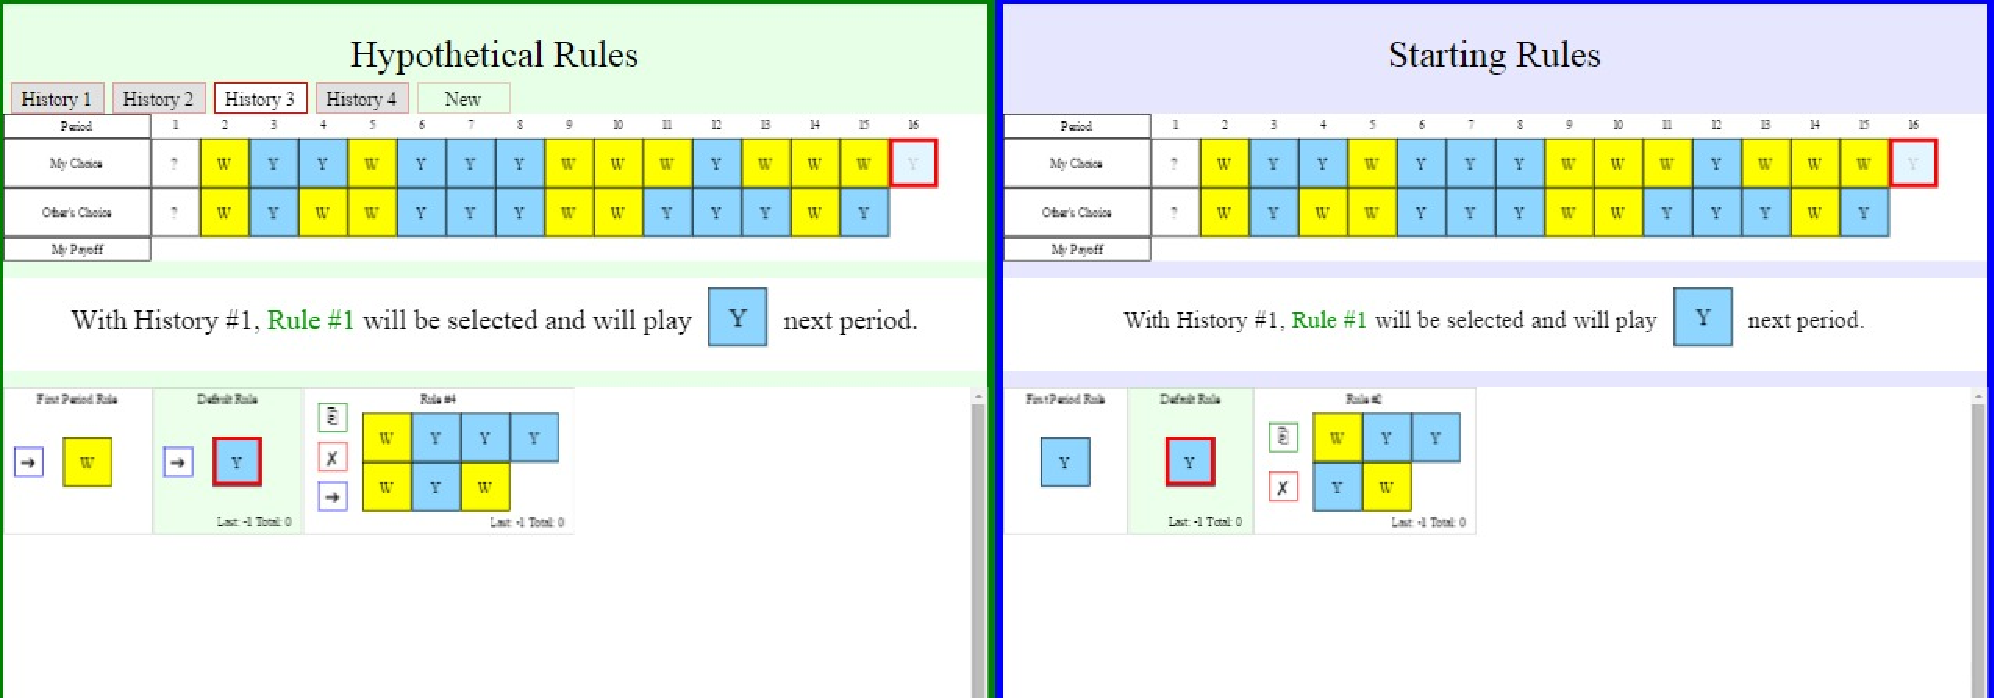
\includegraphics[width=6in]{pictures/splitScreen1.pdf} 

\item \dblbkt{1}Let's look at another example. \dblbkt{1}14 periods of hypothetical History \#3 have been filled in. \dblbkt{1}The hypothetical rule set will play $\secondChoice$ after this history occurs.  \dblbkt{1}The starting rule set will play $\secondChoice$ after this history occurs. \dblbkt{slnc 5000}

\item You will be able to make changes to your Hypothetical Rules, and your Starting Rules, for the duration of the 10 minutes. {\bf After the ten minutes are up, rules that are on the Starting Rules side will be your starting rules for the experiment.}
\end{itemize} 


\subsubsection*{\dblbkt{4}Payoffs} 

 \begin{itemize} 
\item \dblbkt{1}At the end of the experiment, you will be paid in {\bf cash}.   
\item \dblbkt{1}Your payoff at the end of the experiment will be the sum of the payoffs for each period.
\item \dblbkt{1}Reminder, the exchange rate today is \exchangeRate\ Francs = 1 dollar.
\end{itemize} 

\subsection*{\dblbkt{3}Practice Match}
\begin{itemize} 
\item Next, there will be a practice match to make sure that you are comfortable with the interface.
\item It is important to note that in this practice match, 
\begin{itemize} 
\item \dblbkt{1}you will NOT be paid for the choices made.
\item \dblbkt{1}the payoffs are all listed as 0, so that you can focus on getting comfortable with the interface, rather than focusing on the payoffs.
\item \dblbkt{1}You are NOT paired with another participant.  Your opponent for the practice match is a computer that is playing RANDOMLY.
\end{itemize}
\end{itemize} 

%ENDTEXT


\end{document} 



\newpage 
\subsection*{Screenshots}

\hspace{-.5in}
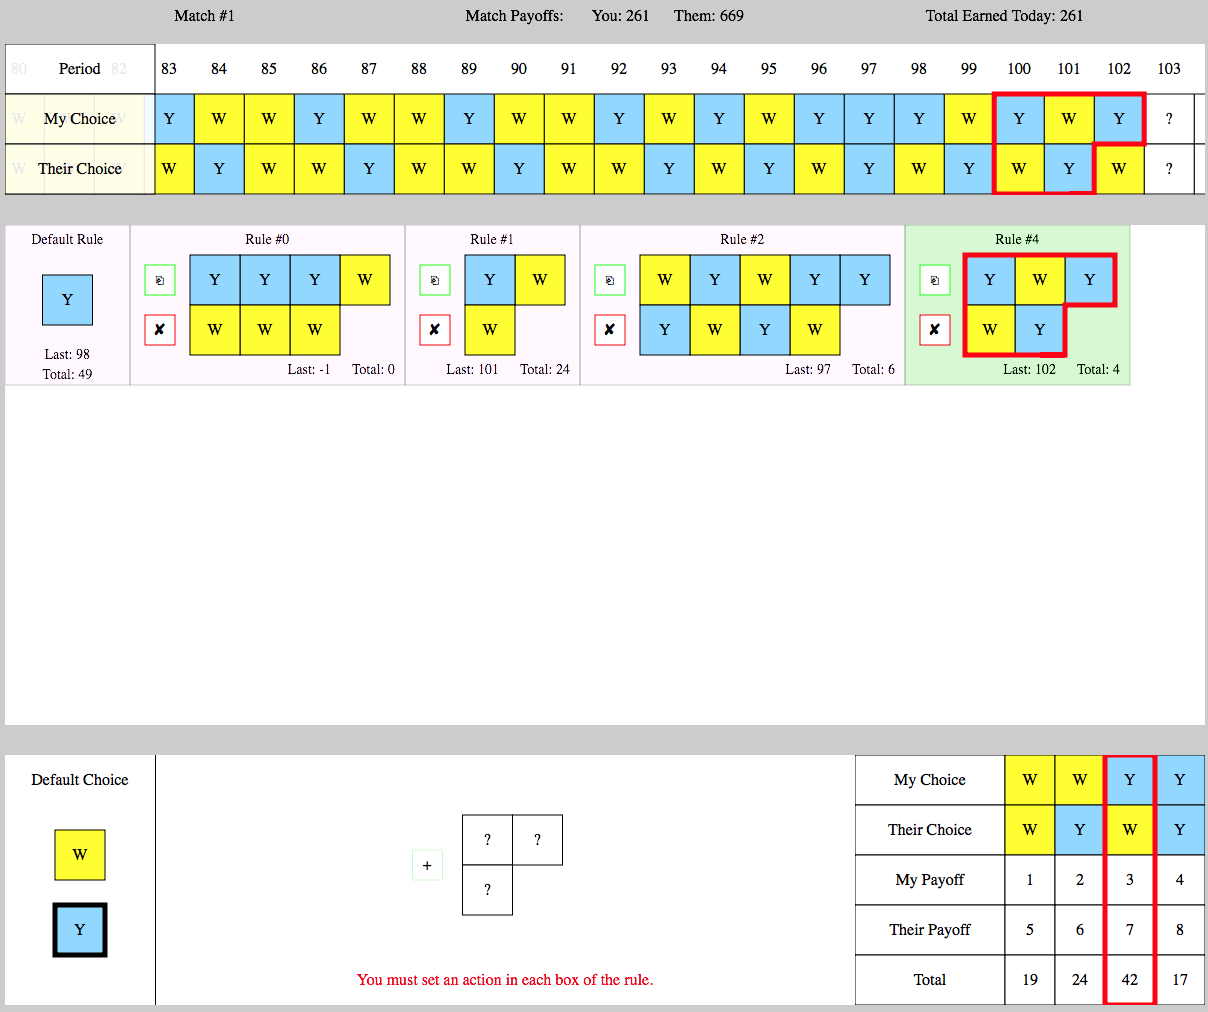
\includegraphics[width=7in]{pictures/ss1.png} 

\begin{itemize} 

\item The history is displayed across the entire screen on the top. 
\item The rule list is displayed in the middle of the screen.
\item The default choice is made in the bottom left, rules can be constructed in the bottom center, and the payoff is displayed in the bottom right.  
\item Notice that the rule that was used to make the most recent choice is highlighted with a green background and is outlined in red on both the rule list and the history.  In the example above, rule \#4 is used to  make the choice in period 102, and therefore that rule is highlighted.  In addition, the payoff in period 102 is highlighted in the game table in the bottom right. 
\end{itemize} 



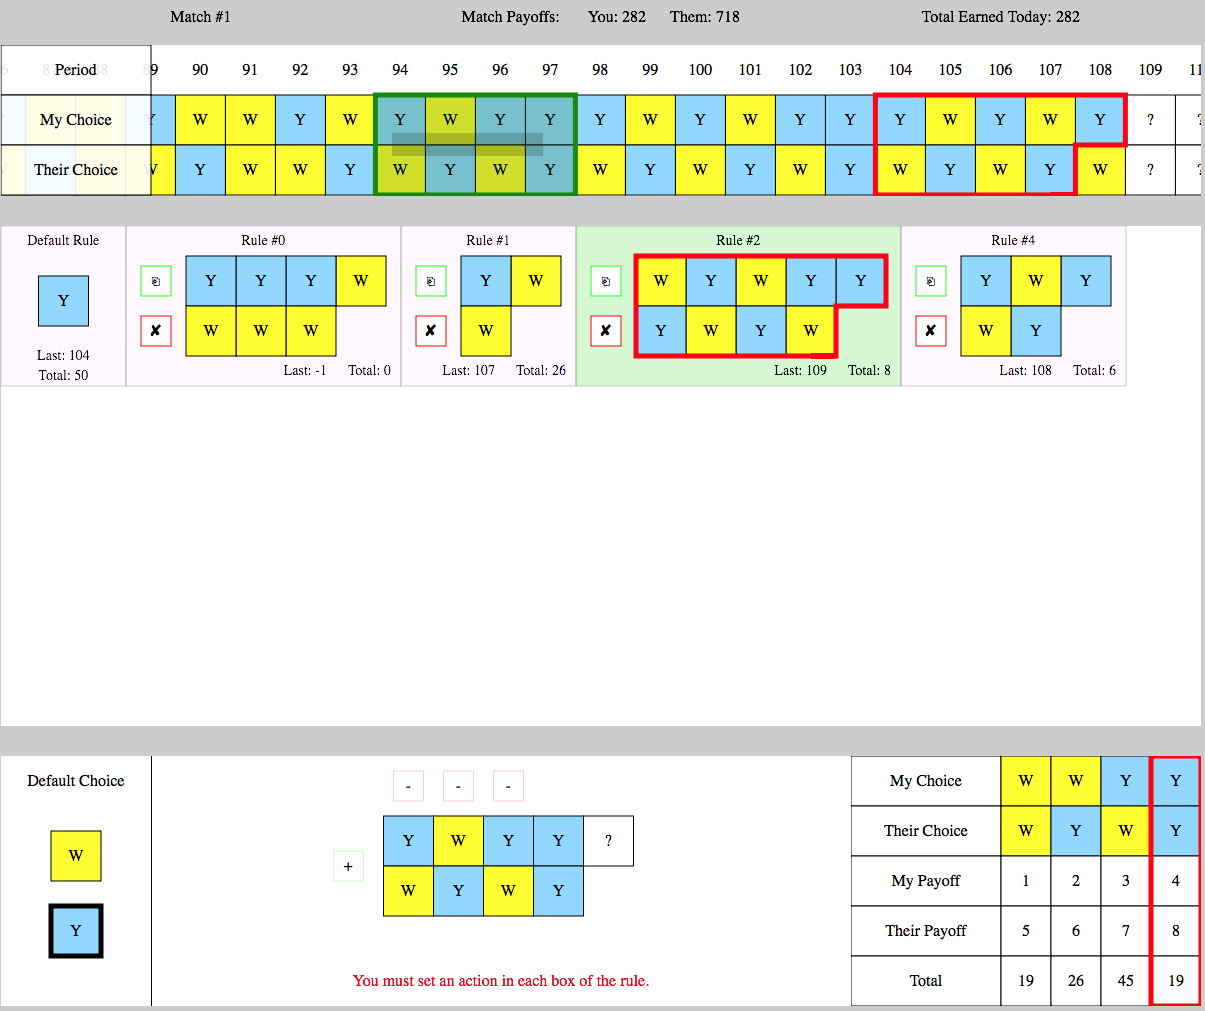
\includegraphics[width=6.5in]{pictures/ss2.png} 
\begin{itemize} 
\item In order to create rules quickly, you can highlight a section of the history and have it appear in the rule constructor as displayed above.  In addition, you can click the constructor area to create other rules (in the screenshot above, periods 94-97 are highlighted and then copied to the bottom center).
\end{itemize} 
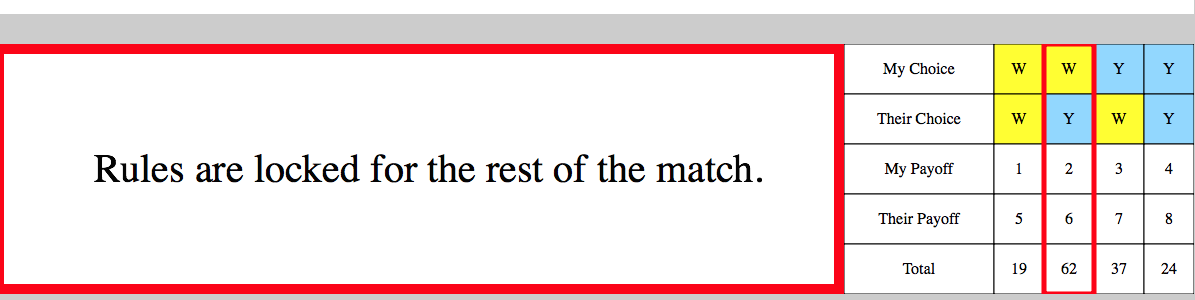
\includegraphics[width=7in]{pictures/ss3.png} 

\begin{itemize} 
\item When the Free Stage ends and the Lock Stage begins, the constructor area will be covered, and you will not be able to make any changes until the Lock Stage ends. 
\end{itemize} 
